\subsection{The action of $\PSL{\Z}$ on $\EC$}

Summing up, the above algorithm allows us to find for a given $z \in \C \setminus \R$ a point $Bz$ which is (under the action of modular group) equivalent to $z$  and which lies in the region $\mathcal{R}$ depicted in Figure~{\ref{fig_SL2FunDomMinRegion}}. By Theorem~\ref{thm_SL2FunDomGlobMin}, statement (\ref{itm_SL2FunDomGlobMinC}), the interior of $\mathcal{R}$ is mapped to itself exactly by transformations $A \in \PSL{\Z}$ with $n(A) = 2$, \ie the identity transformation or $T$. The equivalence of boundary points of $\mathcal{R}$ may be also be established by transformations with $n(A) = 3$, by statement (\ref{itm_SL2FunDomGlobMinB}). It is easy to see that this is indeed the case: The straight line segments of the boundary of $\mathcal{R}$ are equivalent under $U$ or $\inv{U}$ and the two circular arcs bounding $\mathcal{R}$ are equivalent under $TUT$ or $T\inv{U}T$. With these observations, we have nearly reached our goal, a unique representative $z_0 \in \mathcal{R}$ for each equivalence class $[z]_\sim \in \EC/\sim$. But before we define such a system of representatives, we need to make some more definitions.

\index{Extended upper halfplane}
First of all, it is clear that the modular group preserves the upper and lower halfplane and acts symmetrically on them, \ie $A\conj{z} = \conj{Az}$ for all $A \in \PSL{\Z}$ and $z \in \EC$. It is therefore sufficient to consider just one of the two halfplanes, say, the upper halfplane $\mathcal{H} := \setdef{z \in \C}{\Im{z} > 0}$. However, we also want to consider the group action on rational numbers and we therefore define the \emph{extended upper halfplane} $\EU$ as
\begin{equation}
\EU := \setdef{z \in \C}{\Im{z} > 0} \cup \Q \cup \{\infty\}.
\end{equation}

\begin{figure}
\centering
\includegraphics[width=0.8\textwidth]{figures/minimal-region}
\caption{The region $\mathcal{R}$ of numbers $z = u/v \in \EC$ with $\abs{u\conj{v} + \conj{u}v} \le \min\{\abs{u}^2,\abs{v}^2\}$. It is obtained by taking the strip $\setdef{z \in \C}{\Re{z} \in \left[-\reci{2},\reci{2}\right]}$ plus the point $\infty$ and cutting out two open disks of unit radius centered about the real points $\pm 1$. The arising vertices are labeled. As usual, $T$ is the transformation $z \mapsto -\reci{z}$ and $\rho = \exp(2 \pi \ii / 3)$ is a third root of unity.}
\label{fig_SL2FunDomMinRegion}
\end{figure}

\begin{figure}
\centering
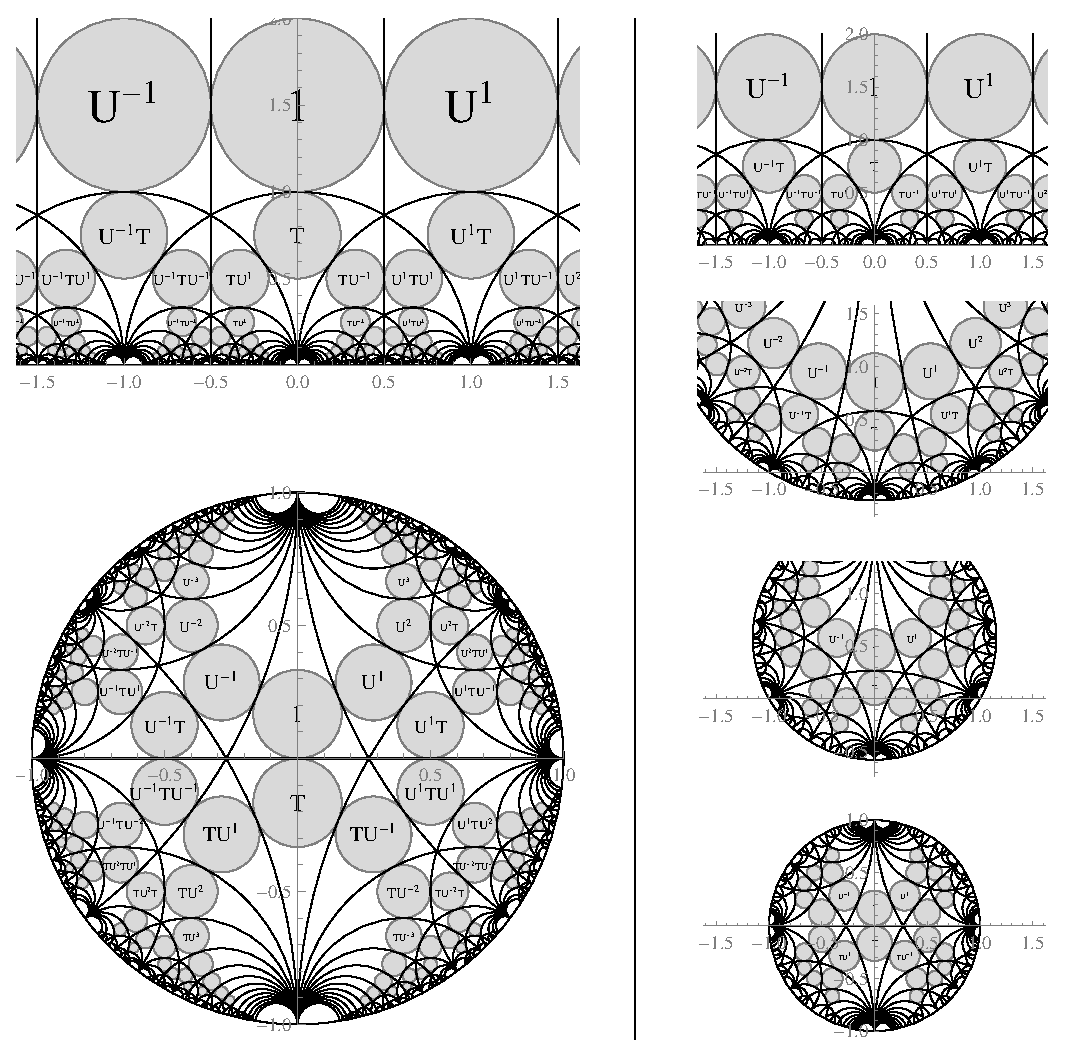
\includegraphics[width=\textwidth]{figures/modular-tiling-1}
\caption{The tessellation of the upper halfplane.}
\label{fig_ModularTiling}
\end{figure}
